\chapter{Space Complexity}

\begin{reference}{Defn}{space}
  (8.1) Let $f:\mathbb N\to \mathbb N$ where $f(n)\geq n$. Say a 1-tape TM $M$ \emph{runs in space} (or the \emph{space complexity} of $M$ is) $f(n)$ iff $M$ always halts and uses at most $f(n)$ tape cells on all inputs of length $n$. Say an NTM $N$ runs in space $f(n)$ iff all branches halt and each branch uses at most $f(n)$ tape cells on all inputs of length $n$.
\end{reference}

\begin{reference}{Defn}{spacecomplexityclass}
  (8.2) Let $f:\mathbb N\to \mathbb R^+$ be a function.
  \begin{align*}
    \mathrm{SPACE}(f(n))  & =\{L|L\text{ is decided by an }O(f(n))\text{ space TM.}\}          \\
    \mathrm{NSPACE}(f(n)) & =\{L|L\text{ is decided by an }O(f(n))\text{ space NTM.}\}\qedhere
  \end{align*}
\end{reference}

\begin{reference}{Defn}{pnpspace}
  (8.6) $\mathrm{PSPACE}=\bigcup_k \mathrm{SPACE}(n^k).$
\end{reference}

\begin{reference}{Thm}{timespace}
  For $t(n)\geq n$,
  \begin{align*}
    \mathrm{TIME}(t(n))  & \subseteq \mathrm{SPACE}(t(n))                                                 \\
    \mathrm{SPACE}(t(n)) & \subseteq \mathrm{TIME}(2^{O(t(n))})=\bigcup_c \mathrm{TIME}(c^{t(n)})\qedhere
  \end{align*}
\end{reference}

\begin{proof}[Proof Sketch]
  A TM that runs in $t(n)$ steps cannot use more than $t(n)$ tape cells. A TM that uses $t(n)$ tape cells cannot use more than $c^{t(n)}$ time without repeating a configuration and looping (for some $c$, for example $c^{t(n)}\leq|\Gamma|^{t(n)}\cdot t(n)\cdot|Q|$).
\end{proof}

\textit{Comment.} $t(n)\geq n$ would be a common assumption, for that we would like to consider bounds that are at least big enough to either read the input (time) or hold the input (space).

\begin{reference}{Cor}{pinpspace}
  $\mathrm{P}\subseteq \mathrm{PSPACE}$.
\end{reference}

\begin{reference}{Thm}{npinpspace}
  $\mathrm{NP}\subseteq \mathrm{PSPACE}$.
\end{reference}

\begin{proof}[Proof Sketch]
  Obviously $\textit{SAT}\in \mathrm{PSPACE}$. Also, if $A\leq_{\mathrm{P}}B$ and $B\in \mathrm{PSPACE}$, then $A\in \mathrm{PSPACE}$, for that it takes polynomial time, thus space by \ref{pinpspace}, to convert $A$ to $B$. Alternatively, we may devise a scheme to try all branches of a NTM in space polynomial to what is required to execute one.
\end{proof}

\begin{reference}{Defn}{conp}
  $\mathrm{coNP}=\{\overline{A}|A\in \mathrm{NP}\}$.
\end{reference}

\begin{reference}{Cor}{conppsapce}
  $\mathrm{coNP}\subseteq \mathrm{PSPACE}$.
\end{reference}

\begin{proof}[Proof Sketch]
  $\mathrm{PSPACE}= \mathrm{coPSPACE}$.
\end{proof}

The complement of any NP-complete language is coNP-complete. (The reduction funcitons are shared.) Below is a figure on a candidate landscape of complexity classes. Interestingly, we do not even know if $\mathrm{P}=\mathrm{PSPACE}$.

\begin{figure}[H]
  \centering
  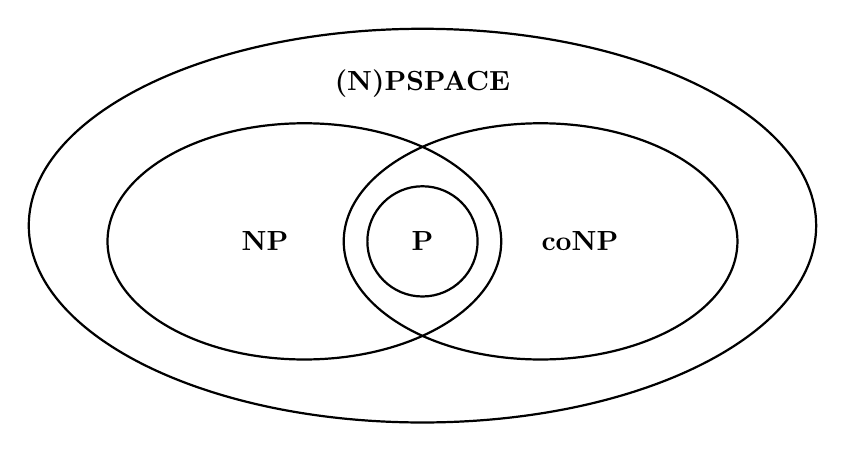
\begin{tikzpicture}

    % PSPACE (outermost oval)
    \draw[thick] (0,0.2) ellipse (5 and 2.5);
    \node at (0,2) {\textbf{(N)PSPACE}};

    % NP
    \draw[thick] (-1.5,0) ellipse (2.5 and 1.5);
    \node at (-2,0) {\textbf{NP}};

    % coNP
    \draw[thick] (1.5,0) ellipse (2.5 and 1.5);
    \node at (2,0) {\textbf{coNP}};

    % P (intersection of NP and coNP)
    \draw[thick] (0,0) ellipse (0.7 and 0.7);
    \node at (0,0) {\textbf{P}};

  \end{tikzpicture}
  \caption{Candidate landscape of complexity classes.}
\end{figure}

\begin{reference}{Defn}{tqbf}
  A \emph{quantified Boolean formula} (QBF) is a Boolean formula with quantifiers that cover all variables. It is very similar to the notion of sentence in logic. A QBF is \texttt{True} or \texttt{False}. $\textit{TQBF}=\{\langle \varphi\rangle|\varphi\text{ is a \texttt{True} QBF}\}$.
\end{reference}

Note that adding existential quantifiers ahead makes \textit{SAT} a special case of \textit{TQBF}.

\begin{reference}{Thm}{tqbfpspace}
  $\textit{TQBF}\in \mathrm{PSPACE}.$
\end{reference}

\begin{proof}[Proof Sketch]
  We remove quantifiers and evaluate the remaining formulas recursively. Each recursive level uses constant space to record the value we plug in. The recursion depth is the number of quantifiers, at most $n=|\langle \varphi\rangle|.$ So $\textit{TQBF}\in \mathrm{SPACE}(n)$.
\end{proof}

\begin{reference}{Defn}{ladderdfa}
  A \emph{ladder} is a sequence of strings of a common length where consecutive strings differ in a single symbol. Let
  \begin{align*}
    \textit{LADDER}_{\mathrm{DFA}}= & \{\langle B,u,v\rangle|B \text{ is a DFA and }L(B)\text{ contains a ladder } \\
                                    & y_1,y_2,\dots,y_k\text{ where }y_1=u\text{ and }y_k=v\}.\qedhere
  \end{align*}
\end{reference}

\begin{reference}{Thm}{ladderdfanpspace}
  $\textit{LADDER}_{\mathrm{DFA}}\in \mathrm{NPSPACE}$.
\end{reference}

\begin{proof}[Proof Sketch]
  We nondeterministically try out all possiblities of variants of $u$ at each step and reject when a variant is not in $L(B)$. We will get this done within $|\Sigma|^{|u|}$ steps and $O(n)$ space.
\end{proof}

\begin{reference}{Thm}{ladderdfapspace}
  $\textit{LADDER}_{\mathrm{DFA}}\in \mathrm{SPACE}(n^2)$.
\end{reference}

\begin{proof}[Proof Sketch]
  We can do this similarly to \ref{acfgp}, which uses DP. Note that we have arbitrarily long time to consume. Write $u\xrightarrow{b}v$ if there exists a ladder from $u$ to $v$ whose length is bounded by $b$. Let $\textit{B-L}=\{\langle B,u,v,b\rangle|B\text{ is a DFA and }u\xrightarrow{b} v\text{ by a ladder in }L(B)\}.$ To decide \textit{B-L}, for $b=1$, accept if $u,v\in L(B)$ differs at at most one place (they could be the same, to allow for a ladder length \textit{bounded by}, not \textit{equals}, $b$), else rejcet. For $b>1$, recursively test $u\xrightarrow{b/2}w$ and $w\xrightarrow{b/2}v$. (If one ladder bounded by $b$ exists, it will be discovered this way.) Now, apply this procedure with $b=|\Sigma|^{|u|}$. The recursion depth is $\log |\Sigma|^{|u|}=O(n)$ and each recursive level uses space $O(n)$ to record $w$, so the total space used is $O(n^2)$.
\end{proof}

\begin{reference}{Thm}{savitch}
  \textbf{SAVITCH}\quad For $f(n)\geq n, \mathrm{NSPACE}(f(n))\subseteq \mathrm{SPACE}(f^2(n))$. (Thus $\mathrm{NPSPACE}=\mathrm{PSPACE}$.)
\end{reference}

\begin{proof}[Proof Sketch]
  We really simply replace ladders in \ref{ladderdfapspace} with tableaus, described in \ref{cooklevin}. So now $u$ and $v$ are configurations, $b$ steps of computation, and $|u|=f(n)$. We then apply this procedure with $b_0=|Q|\times f(n)\times |\Gamma|^{f(n)}$, $u$ the starting configuration and $v$ the accepting configuration. (We can force a single accepting configuration, by for example telling the machine to erase the tape on acceptence and having a single accepting configuration: an empty tape.) Again, each recursion level stores 1 config using space $O(f(n))$. The number of levels would be $\log b_0=O(f(n))$. Thus the total space used is $O(f^2(n))$. To know $f(n)$ on input $w$ given $N$, we simply try $f(n)=1,2,\dots$ using the procedure described until $M$ accepts.
\end{proof}

\begin{reference}{Thm}{pspacecomplete}
  $B$ is \emph{PSPACE-hard} iff for all $A\in \mathrm{PSPACE},A\leq_{\mathrm{P}} B$, and is \emph{PSPACE-complete} if additionally we have $B\in \mathrm{PSPACE}$.
\end{reference}

We are not using $\leq_{\mathrm{PSPACE}}$, for that it will make \textit{every} language in PSPACE PSPACE-complete, thus uninsteresting. In general, we would not like to make reductions too powerful.

\begin{reference}{Thm}{tqbfpspacec}
  \textit{TQBF} is {PSPACE-complete}.
\end{reference}

\begin{proof}[Proof (Attempts)]
  Let $A\in \mathrm{PSPACE}$ be decided by TM $M$ in space $n^k$. Construct $f:w\mapsto \langle \varphi_{M,w}\rangle$ such that $w\in A$ iff $\varphi_{M,w}$ is \texttt{True}. We essentially try to make $\varphi_{M,w}$ say that $M$ accepts $w$, like what we did in \ref{cooklevin}. Yet we cannot use directly the formulas in that proof, for that the formulas will take exponential time to construct (due to our tableau size in this case being $n^k\times |\Sigma|^{n^k}$).

  Instead for configurations $c_i$ and $c_j$, we construct $\varphi_{c_i,c_j,b}$ which says $c_i\xrightarrow{b}c_j$ recursively:
  \[
    \varphi_{c_i,c_j,b}=\exists c_{\text{mid}}\left[\varphi_{c_i,c_{\text{mid}},b/2}\wedge \varphi_{c_{\text{mid}},c_j,b/2}\right].
  \]
  Here $\exists c_{\text{mid}}$ indeed says that there exists such a middle configuration in a fashion same as \ref{cooklevin}. At the base cases where $b=1$, we can use formulas similar to those in \ref{cooklevin} to say that a step is legal. Yet this construction fails again. We are effectively doing no more than \ref{cooklevin}, just fancier, and note that each recursive layer doubles the number of QBFs, so the final outcome is \textit{still} a formula of exponential size (and time)!

  This time we use $\forall$, to avoid the exponentially growing size:
  \[
    \varphi_{c_i,c_j,b}=\exists c_{\text{mid}}\forall(c_g,c_h)\left[\left((c_g,c_h)\in\{(c_i,c_{\text{mid}}),(c_{\text{mid}},c_j)\}\right)\to\varphi_{c_g,c_h,b/2}\right].
  \]
  So same thing is said, except that this time each recursive level adds $O(n^k)$ to the QBF, not doubling its size. The number of levels is $\log |\Gamma|^{n^k}=O(n^k)$, thus the total size is $O(n^{2k})$, and we are done. Note that we did not use the determinism of $M$, and this actually gives a second (yet very same) proof to \ref{savitch}.
\end{proof}

\begin{reference}{Defn}{gg}
  \emph{Generalized Geography Game} is a game played on any directed graph.Players take turns picking nodes that form a simple path. The first player stuck loese.
  \begin{align*}
    \textit{GG}= & \{\langle G,a\rangle|\text{ Player I has a forced win in generalized} \\
                 & \text{geography game on graph }G\text{ starting at node }a\}.\qedhere
  \end{align*}
\end{reference}

\begin{reference}{Thm}{ggpspacecomplete}
  (8.14) \textit{GG} is PSPACE-complete.
\end{reference}

We show this by showing that $\textit{TQBF}\leq_{\mathrm{P}}\textit{GG}$, which is briefly described in \ref{tqbfgg}.

\begin{reference}{Note}{formulagame}
  We define the \emph{Formula Game}: Given QBF $\varphi=\exists x_1\forall x_2\cdots(\forall/\exists x_k)\psi$, consider two players $\exists$ and $\forall$, assigning values to their corresponded variables according to the order of the quantifiers in $\varphi$. Say that $\exists$ wins if the assignment satisfies $\psi$ and otherwise $\forall$ wins. Obviously, $\exists$ has a forced win in the formula game on $\varphi$ iff $\varphi$ is \texttt{True}. Thus $\{\langle \varphi\rangle|\text{ Player }\exists\text{ has a forced win on }\varphi\}=\textit{TQBF}$.
\end{reference}

\begin{reference}{Note}{tqbfgg}
  It turns out we can carefully devise a graph such that the geography game on it essentially mimics the formula game. The complete proof can be found on page 345 of the book.
\end{reference}

\begin{reference}{Defn}{logspace}
  To define sublinear space computation, do not count input as part of space used. Use 2-tape TM model with read-only input tape.
  \begin{align*}
    \mathrm{L}  & =\mathrm{SPACE}(\log n)          \\
    \mathrm{NL} & =\mathrm{NSPACE}(\log n)\qedhere
  \end{align*}
\end{reference}

Log space can represent a constant number of pointers into the input, for that each would take $\log n$ space. Perceive this idea like the internet: We visit the internet through links (pointers), and we never download it as whole.

\begin{reference}{Eg}{eglogn}
  $\{ww^R\}\in \mathrm{L}$, for that we can test the first character is the same as the last, and so forth. $\textit{PATH}\in \mathrm{NL}$, for that we can nondeterministically try out all paths in a graph, keeping in mind only the current node and rejecting a brach if the length of the path is larger than the number of nodes in the graph.
\end{reference}

It is unsolved whether L equals NL.

\begin{reference}{Thm}{linp}
  $\mathrm{L}\subseteq \mathrm{P}$.
\end{reference}

Well, this simply says that \ref{timespace} holds even when $t(n)<n$, and the proof is the same. We only need to define a configuration for $M$ on $w$ seperately (which contains the working tape and the tape head on \textit{both} tapes). Also, by \ref{savitch} we have

\begin{reference}{Thm}{nlspace}
  $\mathrm{NL}\subseteq \mathrm{SPACE}(\log^2n)$.
\end{reference}

Note that $\log n$ is the lower threshold for $f(n)$ or $t(n)$, because with less space than that we cannot access the whole input by any means. In \ref{savitch}, particularly, we needed the space to store \textit{one} configuration (containing \textit{one} tape head on input), and that will already take $\log n$ space.

\begin{reference}{Thm}{nlp}
  $\mathrm{NL}\subseteq \mathrm{P}$.
\end{reference}

\begin{proof}[Proof Sketch]
  Say that NTM $M$ decides $A$ in log space.

  (NL reduction to \textit{PATH} in polynomial time.) Consider a graph $G_{M,w}$ for $M$ on $w$ that has nodes being all configurations for $M$ on $w$ and edges connecting $c_i$ and $c_j$ iff a legal step from $c_i$ to $c_j$ exists. Thus $M$ accepts $w$ iff the $G_{M,w}$ has a path from $c_{\mathrm{start}}$ to $c_{\mathrm{accept}}$. (If we modify $M$ to erase work tape and move heads to left end upon accepting so that there is only one accepting configuration.)

  ($\textit{PATH}\in \mathrm{P}$.) Now on input $w$, we construct $G_{M,w}$, which has a polynomial size and thus takes polynomial time to construct, and search for paths from $c_{\mathrm{start}}$ to $c_{\mathrm{accept}}$, which also takes polynomial time.
\end{proof}

\begin{reference}{Defn}{nlcomplete}
  $B$ is NL-complete iff $B\in \mathrm{NL}$ and $\forall A\in \mathrm{NL}, A\leq_{\mathrm{L}}B$.
\end{reference}

\begin{reference}{Defn}{logtransducer}
  A \emph{log-space transducer} is a TM with three tapes: a read-only input tape of size $n$, a work tape of size $O(\log n)$, and a write-only output tape. $\leq_{\mathrm{L}}$ is defined using this notion.
\end{reference}

\begin{reference}{Thm}{logreduction}
  If $A\leq_{\mathrm{L}}B$ and $B\in \mathrm{L}$, then $A\in \mathrm{L}$.
\end{reference}

\begin{proof}[Proof Sketch]
  This is surprisingly not obvious for that $f(w)$ might cost us more than log space. A workaround is that we compute individual symbols of $f(w)$ that the decider for $B$ requires at each computing step. So we may re-compute $f(w)$.
\end{proof}

\begin{reference}{Note}{npreducinlog}
  All typical NP-complete reductions can be done in log space.
\end{reference}

\begin{reference}{Thm}{pathnlcomplete}
  \textit{PATH} is NL-complete.
\end{reference}

\begin{proof}[Proof Sketch]
  So we really want to make the reduction in \ref{nlp} a log-space one. To achieve this, we go over all possible \textit{pairs} of configurations in some order and see if any of them makes a legal step in $M$. If one do print it as an edge.
\end{proof}

\begin{reference}{Thm}{com2satnlcomp}
  $\overline{2 \textit{SAT}}$ is NL-complete.
\end{reference}

\begin{proof}[Proof Sketch]
  We show that $\textit{PATH}\leq_{\mathrm{L}}\overline{2 \textit{SAT}}$. For each node $u$ in $G$ put a variable $x_u$ in $\varphi$. For each edge $(u,v)$ in $G$ put a clause $(x_u\to x_v)$ in $\varphi$. In addition put the clauses $(x_s\vee x_s)$ and $(x_s\to \overline{x_t})$ in $\varphi$.Thus if $\varphi$ is unsatisfiable, we conclude that path from $s$ to $t$ exists. Similarly, we have that $\overline{2 \textit{SAT}}\in \mathrm{NL}$, by nondeterministically guessing a starting variable $x_u$ and again guessing a path, where each step is one of the clauses transformed as $(x_i\to x_j)$ to derive a contradiction.

  In both parts, if contradictions do not exist, we can assign truth values to variables accordingly to satisfy $\varphi$. (For the second part, assign each variable a node to see that it is exactly the same as the first part.) That said, we state informally that graphs and 2\textit{SAT} formulas are \textit{isomorphic}.
\end{proof}

\begin{reference}{Notes}{nlcertificates}
  NL is the class of languages that are log space verifiable. Cf. \ref{npverify}.
\end{reference}

\begin{reference}{Thm}{nlconl}
  \textbf{Immerman-Szelepcs\'enyi}\quad $\mathrm{NL}=\mathrm{coNL}$.
\end{reference}

\begin{proof}[Proof Sketch]
  It suffices to show that $\overline{\textit{PATH}}\in \mathrm{NL}$, which in turn reduces to computing $path$, defined as follows.
  \begin{reference}{Defn}{ntmcompute}
    NTM $M$ computes function $f$ if for all $w$, if all branches of $M$ on $w$ halt with $f(w)$ on the tape or reject and some branch does not reject.
  \end{reference}
  Let $path(\langle G,s,t\rangle)=\begin{cases}\text{YES,}&\text{if $G$ has path from $s$ to $t$,}\\ \text{NO,}&\text{if not.}\end{cases}$.\newline
  Let $R(G,s)=\{u|path(\langle G,s,u\rangle)=\text{YES}\},c(\langle G,s\rangle)=|R(G,s)|,$ and $m$ be the number of nodes in $G$.
  \begin{reference}{Lem}{pathtoc}
    If some log-space NTM computes $path$, then another computes $c$.
  \end{reference}
  \begin{proof}[Proof Sketch]
    We simply go over all nodes and count. Computing $path$ can turn out unsuccessful on some branchs, yet \textit{some} branch will successfully compute all paths and produce the right answer. Conversely,
  \end{proof}
  \begin{reference}{Lem}{ctopath}
    If some log-space NTM computes $c$, then another computes $path$.
  \end{reference}
  \begin{proof}
    We effectively guess all $c$ nodes and see if $t$ is among them. The formal description of this process can appear a bit techical to correctly capture the notion of nondeterminism.
    \begin{align*}
      {``} & \text{ On input }\langle G,s,t\rangle                                                      \\
      1.   & \text{ Compute }c\text{ and set }k\leftarrow0.                                             \\
      2.   & \text{ For each node $u$, nondeterministically go to (a) or (b):}                          \\
           & \text{ (a) Nondeternimistically pick a path from $s$ to $u$ with length no more than $m$.} \\
           & \quad\quad\text{If fail, \textit{reject}.}                                                 \\
           & \quad\quad\text{Else }  \begin{aligned}[t]
                                        & \text{If $u=t$, then \textit{output} YES.} \\
                                        & \text{Else set }k\leftarrow k+1.
                                     \end{aligned}              \\
           & \text{ (b) Skip $u$ and continue.}                                                         \\
      3.   & \text{ If $k\neq c$, \textit{reject}. Else \textit{output} NO.''}\qedhere
    \end{align*}
  \end{proof}
  Switching gears!

  Let $path_d(\langle G,s,t\rangle)=\begin{cases}\text{YES,}&\text{if $G$ has a path of length $\leq d$ from $s$ to $t$,}\\ \text{NO,}&\text{if not.}\end{cases}$\newline
  Let $R_d(G,s)=\{u|path_d(\langle G,s,u\rangle)=\text{YES}\}$ and $c_d(\langle G,s\rangle)=|R_d(G,s)|$.

  Now, with almost the same proof, we have:
  \begin{reference}{Cor}{pathdtocd}
    If some log-space NTM computes $path_d$, then another computes $c_d$.
  \end{reference}
  Altering the proof of \ref{ctopath} a little bit, changing ``If $u=t$'' to ``If $u$ has an edge to $t$'', we obtain:
  \begin{reference}{Cor}{cdtopathd}
    If some log-space NTM computes $c_d$, then another computes $path_{d+1}$.
  \end{reference}
  By the two corollaries above,
  \begin{reference}{Cor}{cdtocdpo}
    We can use a log-space NTM that computes $path_d$ to compute $path_{d+1}$.
  \end{reference}
  Then we compute $path_1$ all the way to $path_m$, and that is all we need.
\end{proof}

$\overline{2 \textit{SAT}}$ is NL-complete, so it is coNL-complete, thus $2 \textit{SAT}$ is NL-complete.

\section*{Exercises and Problems}

\setcounter{exercise}{7}

\begin{exercise}
  Question to fill in.
\end{exercise}

\textcolor{red}{to do}

\begin{exercise}
  \ref{ladderdfapspace}.
\end{exercise}

See \ref{ladderdfapspace}.

\begin{exercise}
  Question to fill in.
\end{exercise}

\textcolor{red}{to do}

\setcounter{exercise}{12}

\begin{exercise}
  Question to fill in.
\end{exercise}

\textcolor{red}{to do}

\begin{exercise}
  Question to fill in.
\end{exercise}

\textcolor{red}{to do}

\setcounter{exercise}{21}

\begin{exercise}
  Question to fill in.
\end{exercise}

\textcolor{red}{to do}

\setcounter{exercise}{26}

\begin{exercise}
  Question to fill in.
\end{exercise}

\textcolor{red}{to do}
